% !TeX spellcheck = ru_RU
\chapter{Исследовательская часть}

В данном разделе будут описаны технические характеристики устройства, на котором проводилось измерение времени работы ПО, а также представлены результаты измерения времени работы реализаций алгоритмов.

\section{Технические характеристики}

Ниже приведены технические характеристики устройства, на котором было проведено измерение времени работы ПО:

\begin{itemize}
    \item операционная система Windows 10 Домашняя Версия 21H1 \cite{windows} x86\_64;
    \item оперативная память 8 Гб 2133 МГц;
    \item процессор Intel Core i5-8300H с тактовой частотой 2.30ГГц \cite{intel}.
\end{itemize}

При тестировании ноутбук был включен в сеть электропитания и был нагружен только системой тестирования и встроенными приложениями окружения.

\section{Время выполнения реализаций алгоритмов}

Для замеров времени используется функция замера процессорного времени process\_time из библиотеки time на Python. Функция возвращает процессорное время типа float \cite{time}.

Функция используется дважды --- в начале и в конце замера времени, затем значения начальное значение вычитается из конечного.

При сравнительной оценке рассмотренных алгоритмов стоит учитывать, что ни отсортированный по возрастанию, ни отсортированный по убыванию массив не являются худшим случаем для алгоритма блочной сортировки. Рассмотрим результаты работы алгоритмов блочной и пирамидальной сортировки на массиве с неравномерным распределением чисел на отрезке $[A_{min}, A_{max}]$, где  $A_{min}$ и  $A_{max}$ являются наименьшим и наибольшим значениями в массиве A. Для каждой длины массива $N$ был сгенерирован массив, $N-1$ элементов которого принадлежат в промежутку [0, 1], а последний элемент равен 1000000. При таком распределении чисел в алгоритме блочной сортировки $N-1$ попадут в первый блок, что существенно повысит трудоемкость сортировки этого блока. Последний элемент массива попадет в последний блок, все остальные блоки останутся пустыми.

Результаты замеров времени реализаций алгоритмов приведены в таблицах \ref{tbl:sorted} --- \ref{tbl:bad}.

\begin{table}[h]
	\captionsetup{justification=raggedright,singlelinecheck=off}
	\caption{Результаты замеров времени работы реализаций сортировок на отсортированных по возрастанию массивах (в мсек)}
	\label{tbl:sorted}
	\centering
	\begin{tabular}{|c|c|c|c|c|}\hline%
		Размер & Пузырьком &  Пирамидальная &  Блочная
		\csvreader[head to column names]{csv/sorted.csv}{}%
		{\\ \hline\len & \bubble & \heap & \bucket}%
		\\ \hline
	\end{tabular}
\end{table}

\begin{table}[h]
	\captionsetup{justification=raggedright,singlelinecheck=off}
	\caption{Результаты замеров времени работы реализаций сортировок на отсортированных по убыванию массивах (в мсек)}
	\label{tbl:dec}
	\centering
	\begin{tabular}{|c|c|c|c|c|}\hline%
		Размер & Пузырьком &  Пирамидальная &  Блочная
		\csvreader[head to column names]{csv/sorted.csv}{}%
		{\\ \hline\len & \bubble & \heap & \bucket}%
		\\ \hline
	\end{tabular}
\end{table}


\begin{table}[h]
	\captionsetup{justification=raggedright,singlelinecheck=off}
	\caption{Результаты замеров времени работы реализаций сортировок на массивах, заполненных случайными числами (в мсек)}
	\label{tbl:rand}
	\centering 
	\begin{tabular}{|c|c|c|c|c|}\hline%
		Размер & Пузырьком &  Пирамидальная &  Блочная
		\csvreader[head to column names]{csv/random.csv}{}%
		{\\ \hline\len & \bubble & \heap & \bucket}%
		\\ \hline
	\end{tabular}
\end{table}


\begin{table}[h]
	\captionsetup{justification=raggedright,singlelinecheck=off}
	\caption{Результаты замеров времени работы реализаций сортировок на массивах c неравномерным распределением данных (в мсек)}
	\label{tbl:bad}
	\centering 
	\begin{tabular}{|c|c|c|c|c|}\hline%
		Размер & Пузырьком &  Пирамидальная &  Блочная
		\csvreader[head to column names]{csv/random.csv}{}%
		{\\ \hline\len & \bubble & \heap & \bucket}%
		\\ \hline
	\end{tabular}
\end{table}
\clearpage
На рисунках \ref{img:sorted_all} --- \ref{img:rand_two} приведена графическая интерпретация полученных замеров времени.

\begin{figure}[h]
	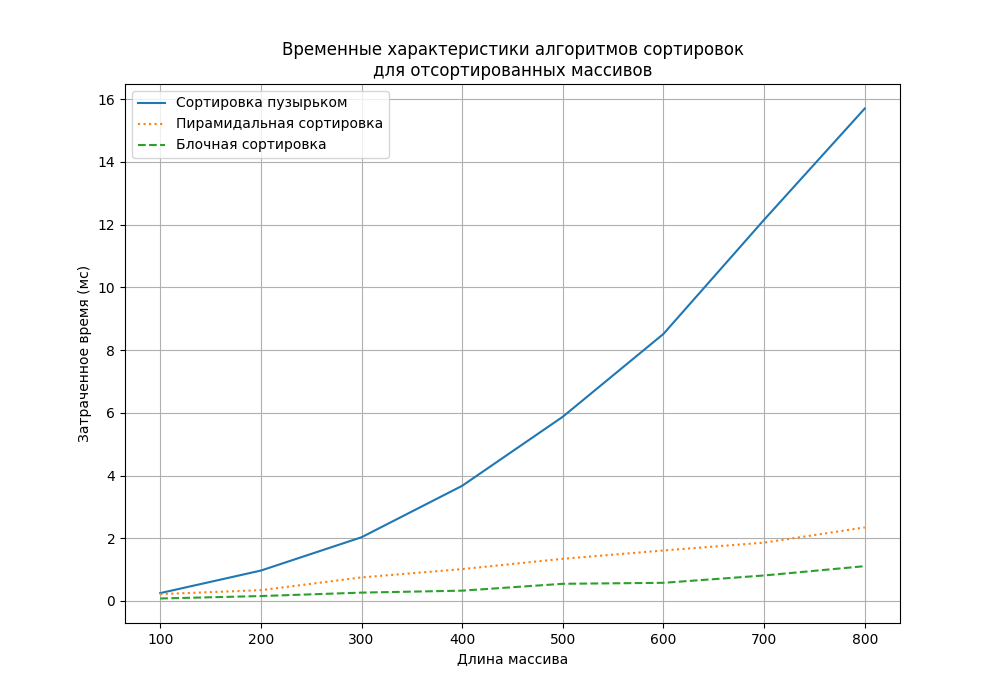
\includegraphics[scale=0.45]{img/sorted.png}
	\centering 
	\caption{Результаты замеров времени работы реализаций сортировок на отсортированных по возрастанию массивах}
	\label{img:sorted_all}
\end{figure}
\begin{figure}[h]
	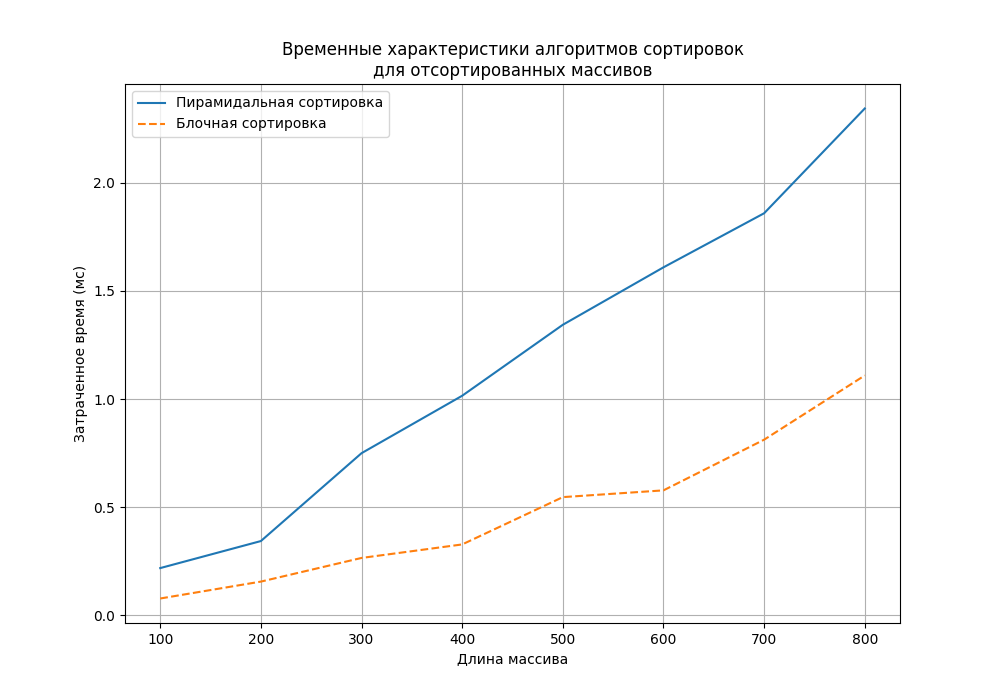
\includegraphics[scale=0.45]{img/sorted_two.png}
	\centering 
	\caption{Результаты замеров времени работы реализаций сортировок на отсортированных по возрастанию массивах}
	\label{img:sorted_two}
\end{figure}
\begin{figure}[h]
	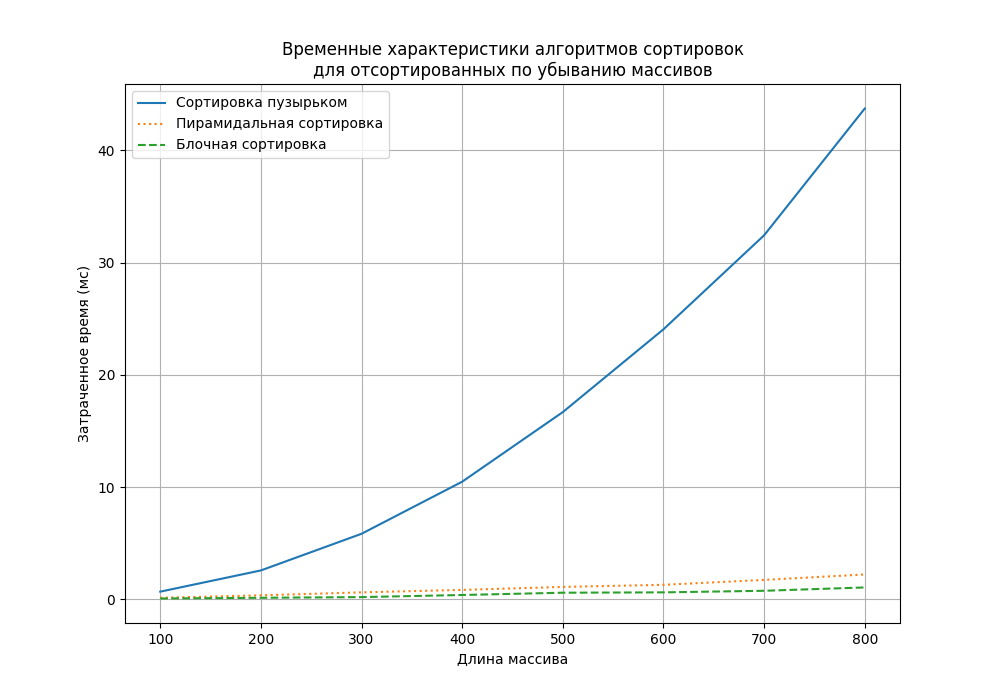
\includegraphics[scale=0.5]{img/dec.png}
	\centering 
	\caption{Результаты замеров времени работы реализаций сортировок на отсортированных по убыванию массивах}
	\label{img:dec_all}
\end{figure}
\begin{figure}[h]
	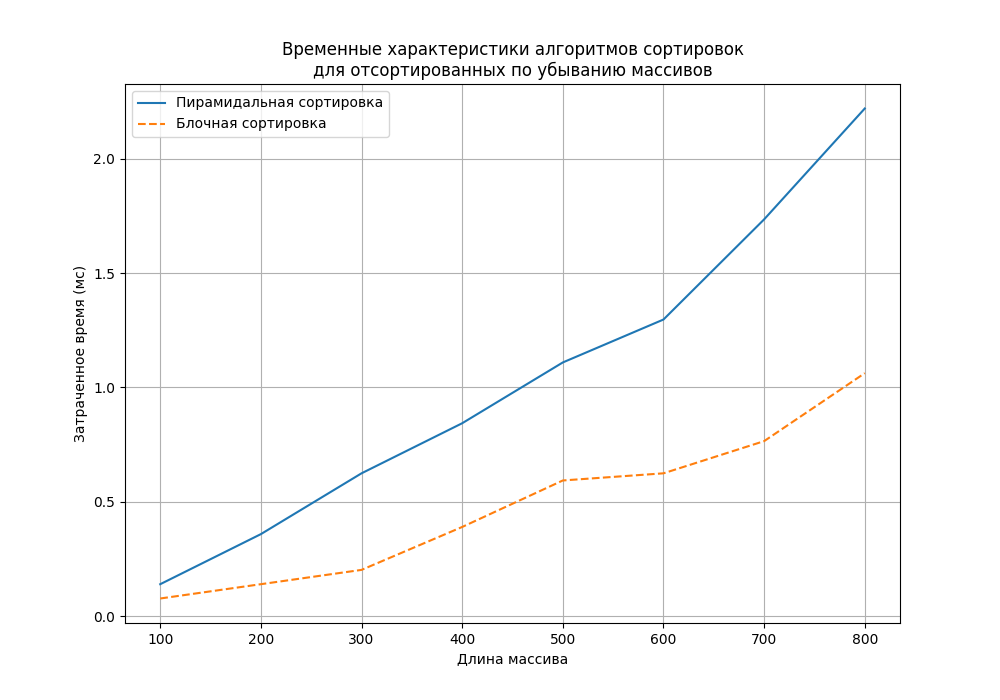
\includegraphics[scale=0.5]{img/dec_two.png}
	\centering 
	\caption{Результаты замеров времени работы реализаций сортировок на массивах, заполненных случайными числами}
	\label{img:dec_two}
\end{figure}
\begin{figure}[h]
	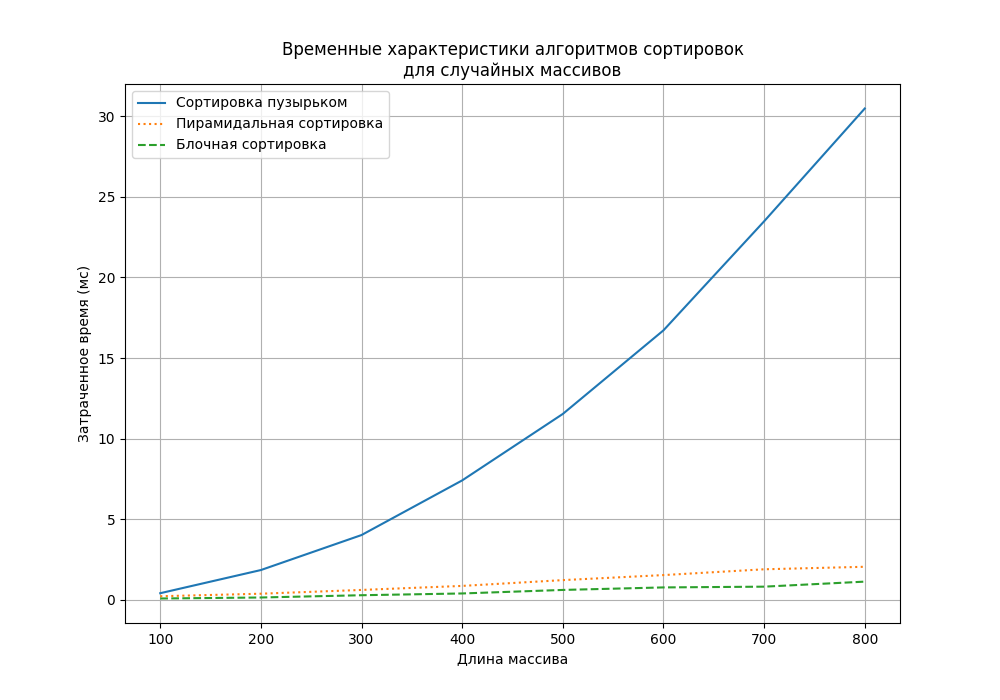
\includegraphics[scale=0.5]{img/random.png}
	\centering 
	\caption{Результаты замеров времени работы реализаций сортировок на массивах, заполненных случайными числами}
	\label{img:rand_all}
\end{figure}

\begin{figure}[h]
	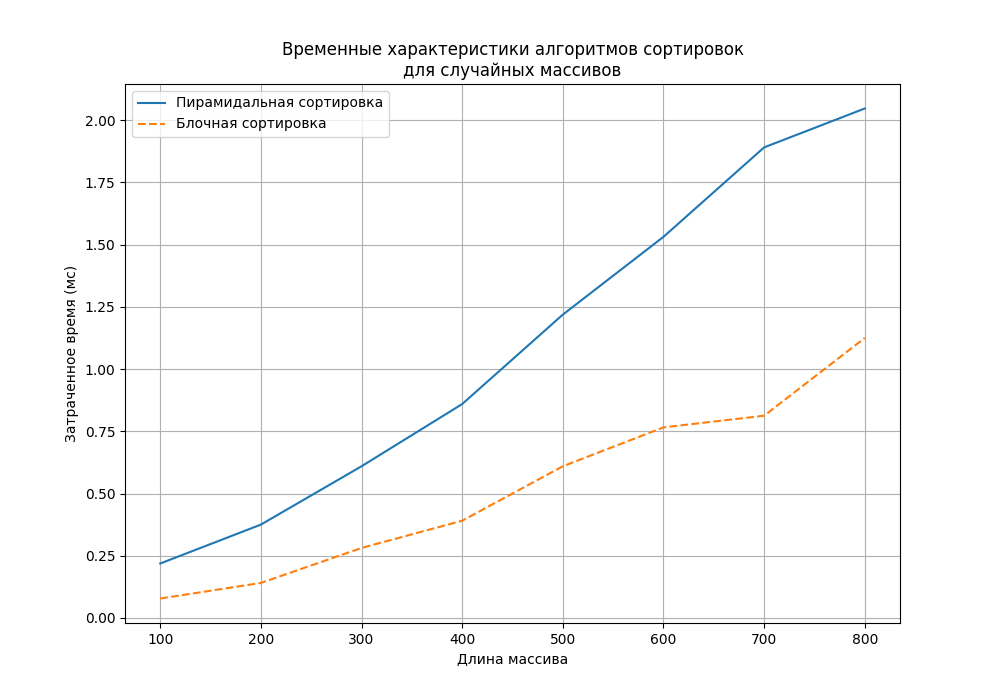
\includegraphics[scale=0.5]{img/random_two.png}
	\centering 
	\caption{Результаты замеров времени работы реализаций сортировок на отсортированных по возрастанию массивах}
	\label{img:rand_two}
\end{figure}

\begin{figure}[h]
	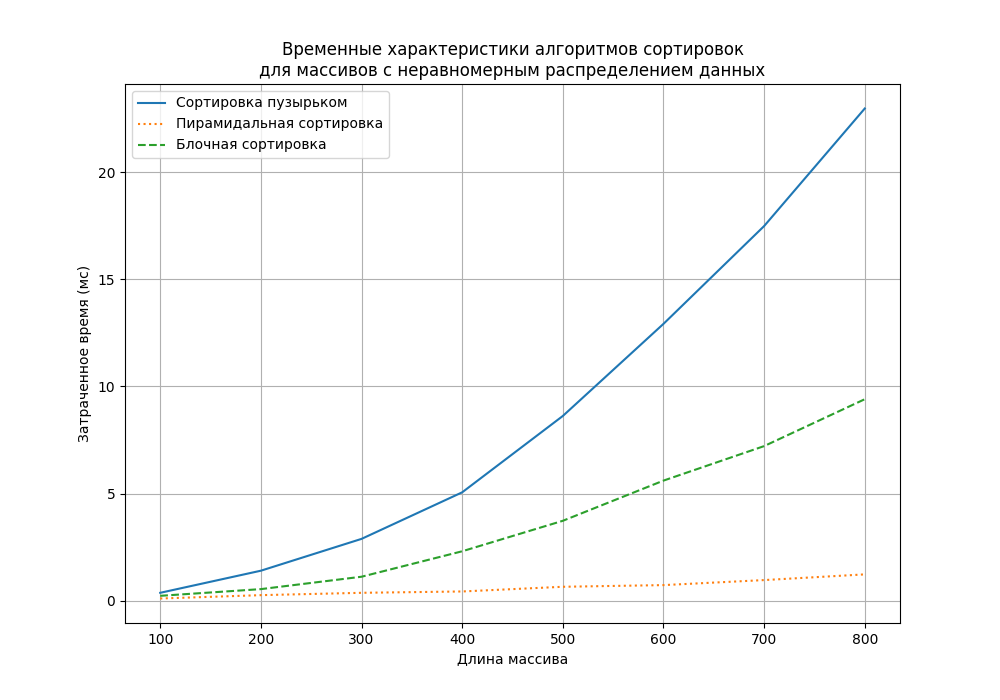
\includegraphics[scale=0.5]{img/bad.png}
	\centering 
	\caption{Результаты замеров времени работы реализаций сортировок на массивах с неравномерным распределением данных}
	\label{img:bad_all}
\end{figure}

\begin{figure}[h]
	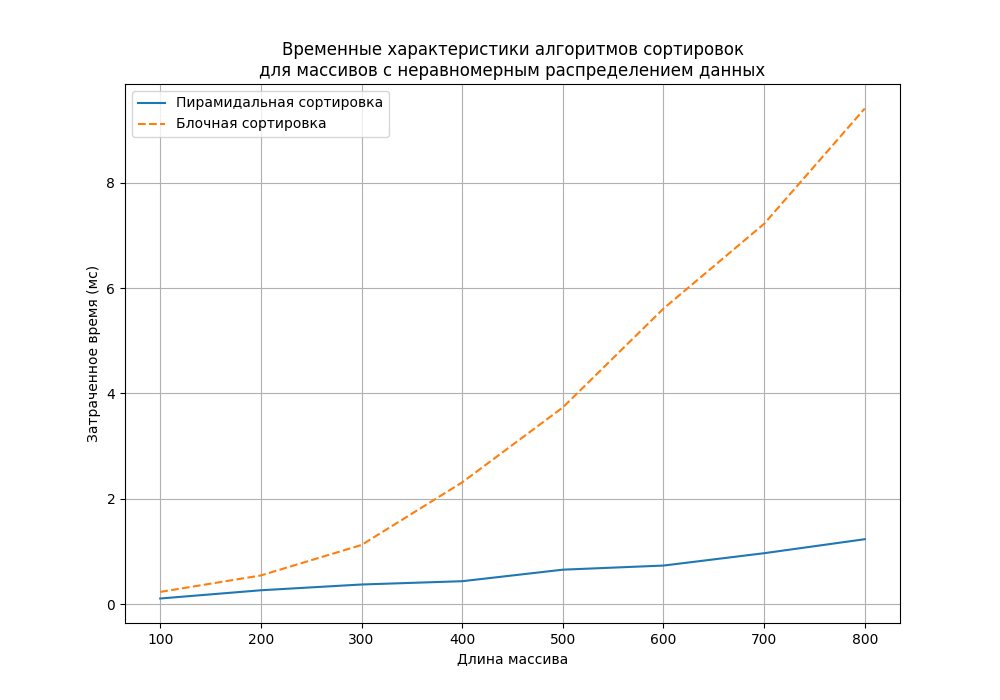
\includegraphics[scale=0.5]{img/bad_two.png}
	\centering 
	\caption{Результаты замеров времени работы реализаций сортировок на массивах с неравномерным распределением данных}
	\label{img:bad_two}
\end{figure}
\clearpage
Сортировка пузырьком работает дольше других рассмотренных сортировок на любых массивах. 

Для любых массивов с равномерным распределением данных блочная сортировка работает быстрее, чем пирамидальная (Рис. \ref{img:sorted_two}, \ref{img:dec_two}, \ref{img:rand_two}). В случаях неравномерного распределения чисел в массиве блочная сортировка проигрывает пирамидальной, но все еще работает быстрее сортировки пузырьком (Рис. \ref{img:bad_all}).
\section*{Вывод}
Исходя из полученных результатов, сортировка пузырьком является наиболее долгой из всех рассмотренных алгоритмов (для массива длины 800 примерно в 15-20 раз дольше блочной сортировки). Для любых массивов с равномерным распределением данных, блочная сортировка работает быстрее пирамидальной. В случае неравного распределения данных большая часть блоков в алгоритме блочной сортировки остаются незадействованы, что негативно сказывается на времени сортировки. В таких случаях пирамидальная сортировка работает быстрее блочной.

Можно сделать вывод, что использование блочной сортировки является более предпочтительным для сортировки данных, полученных в результате какого-то случайного процесса (как правило результаты такого процесса будут равномерно распределены на отрезке от минимального до максимального значения в массиве). В случаях, когда данные в массиве заведомо распределены неравномерно, предпочтительнее использование пирамидальной сортировки.

Теоретические результаты оценки трудоемкости и полученные практическим образом результаты замеров совпадают.



